\documentclass{beamer}

\mode<presentation>
{
\usetheme{CambridgeUS}
\usecolortheme[rgb={0.64, 0, 0}]{structure}

%\setbeamercovered{transparent}
%\useinnertheme{circles}

\setbeamertemplate{navigation symbols}{}
}

\usepackage{ngerman}
\usepackage[ngerman]{babel}
\usepackage[utf8]{inputenc}% UTF8-Kodierung für Umlaute usw
\usepackage[T1]{fontenc}

\usepackage{color} % Farben
\usepackage{microtype} % spezielle PDF-mikrotypographische Optimierungen
\usepackage{graphicx} % Bilder
\usepackage{multimedia}

\title[Bedeutungen]
{Die Bedeutung der Bedeutungen unter besonderer Berücksichtigung der Bedeutungen}
\author{Max Mustermann} 
\institute[Arbeit]{Vortrag Arbeit\\beim Birnbaum-Institut}
\date{1.1.2014} % Importiere die Einstellungen aus der Präambel
\begin{document}

\begin{frame}
	\titlepage
\end{frame}


\section{Einleitung}


\begin{frame}{Bedeutungen}
	\begin{itemize}
		\item<1-> dieser Punkt ist die ganze Zeit sichtbar
		\item<2> dieser Punkt ist nur beim zweiten Teil sichtbar
		\item<3> dieser Punkt ist erst beim dritten Teil sichtbar
		\item<3> dieser Punkt ist erst beim dritten Teil sichtbar
		\end{itemize}
\end{frame}


\begin{frame}{Gliederung}
	\tableofcontents[sections={<2->},firstsection=2]
\end{frame}

\section{Sektion 1}
\subsection{Untersektion 1}
\begin{frame}{Gleichung}
	\begin{itemize}
		\item Natürlich können hier alle Fähigkeiten von \LaTeX\, genutzt werden.
	\end{itemize}
	\begin{equation}
		a^2 + b^2 = c^2
	\end{equation}
\end{frame}


\begin{frame}{Abbildungen}
	\begin{columns}
		\begin{column}{0.5\linewidth}
			\begin{itemize}
				\item blabla bla 
				\item blabla bla 	
			\end{itemize}
		\end{column}
		\begin{column}{0.5\linewidth}
			\centering{ein Bild folgt}
			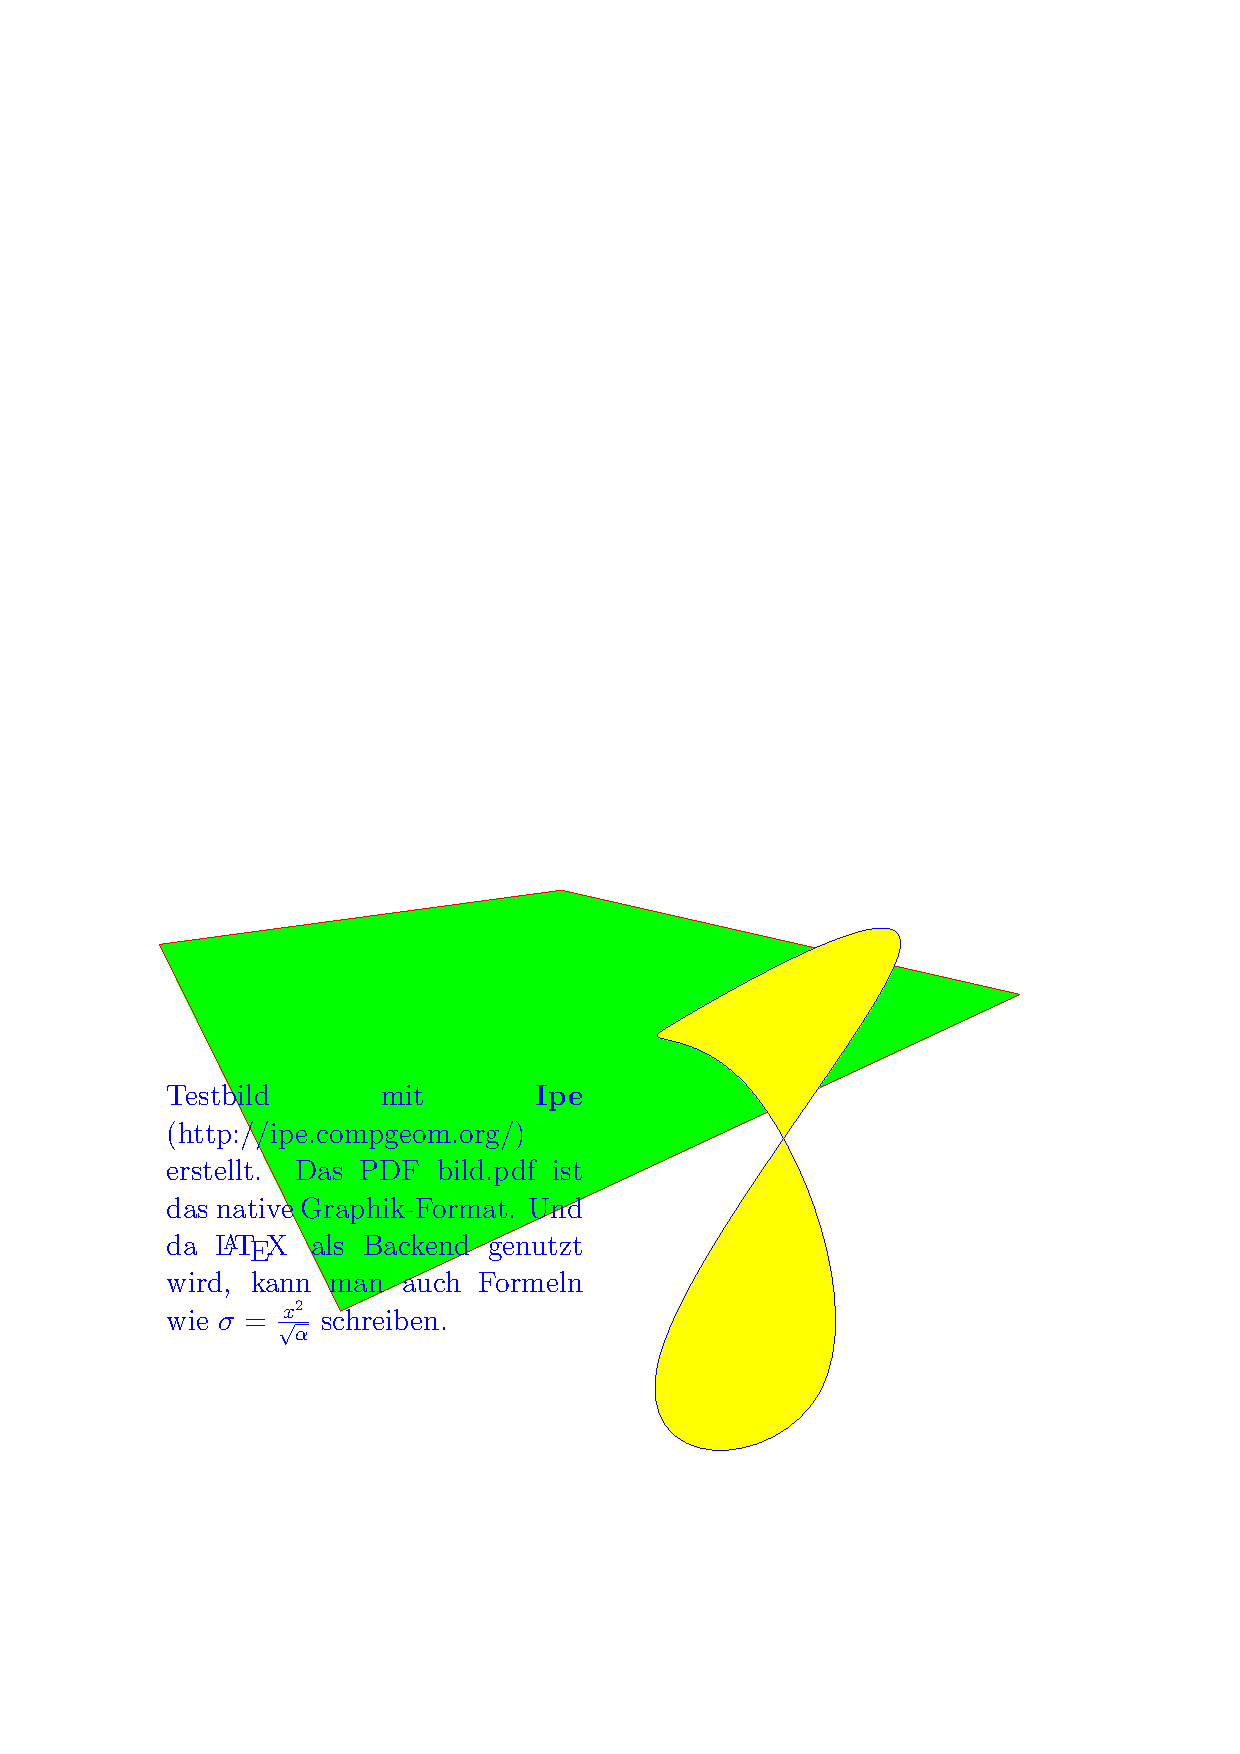
\includegraphics[width=1\linewidth]{images/bild}
		\end{column}		
	\end{columns}

	\begin{equation}
		a^2 + b^2 = c^2
	\end{equation}
\end{frame}



\section{Zusammenfassung}

\begin{frame}{Zusammenfassung}
	\begin{itemize}
		\item Blau ist die Farbe
	\end{itemize}
	\begin{block}{Ausblick}
	\begin{itemize}
		\item Blau kann mit verschiedenen Farben gemischt werden
		\item Vieles wird erst bei tiefgründiger Betrachtung sichtbar werden
	\end{itemize}		
	\end{block}
\end{frame}



\begin{frame}
	\frametitle{Diskussion}
	\begin{center}
 		Vielen Dank für Ihre Aufmerksamkeit!
	\end{center}
\end{frame}

\end{document}